\subsection{Эмпирическая функция распределения}

\subsubsection{Вариационный ряд}

Если упорядочить выборку по неубыванию, получим \textit{вариационный ряд}:

\begin{table}[h!]
\centering
\begin{tabular}{|c|c||c|c||c|c||c|c|}
\hline
$i$ & $x_{(i)}$ & $i$ & $x_{(i)}$ & $i$ & $x_{(i)}$ & $i$ & $x_{(i)}$ \\ \hline \hline
1 & 2.55 & 6 & 3.01 & 11 & 3.12 & 16 & 3.30 \\ \hline
2 & 2.66 & 7 & 3.03 & 12 & 3.14 & 17 & 3.32 \\ \hline
3 & 2.89 & 8 & 3.05 & 13 & 3.21 & 18 & 3.34 \\ \hline
4 & 2.89 & 9 & 3.07 & 14 & 3.24 & 19 & 3.38 \\ \hline
5 & 2.95 & 10 & 3.09 & 15 & 3.25 & 20 & 3.42 \\ \hline
\end{tabular}
\caption{Вариационный ряд}
\end{table}

\subsubsection{График функции}

По определению эмпирической функции распределения:
\[
    \hat{F}(x)=\dfrac{1}{n}\sum_{i=1}^n\mathbf{1}_{\{X_i<x\}},
\]

где \( \mathbf{1}_{\{X_i<x\}} \) --- индикаторная функция события \( \{X_i< x\} \), \( x\in\mathbb{R} \).

Для построения графика функции воспользуемся библиотекой \textit{TiKZ}. Чтобы автоматизировать процесс и избежать риска ошибки, напишем скрипт:
\begin{lstlisting}[caption=Функция построения графика]
def generate_plot(variation_series):
  # draw first line
  result = tikz_header
  result += r"\addplot[ultra thick, black, no marks, const plot] coordinates {"
  result += f"(2.5, 0) "
  result += f"({variation_series[0]}, 0)"
  result += "};\n"
  result += r"\addplot[only marks, mark=*, mark options={fill=black}, mark size=2pt] coordinates {"
  result += f"({variation_series[0]}, 0)"
  result += "};\n"
  # draw last line
  result += r"\addplot[ultra thick, black, no marks, const plot] coordinates {"
  result += f"({variation_series[n-1]}, 1) "
  result += f"(3.5, 1)"
  result += "};\n"
  result += r"\addplot[only marks, mark=*, mark options={fill=white, draw=black}, mark size=2pt] coordinates {"
  result += f"({variation_series[n-1]}, 1)"
  result += "};\n"
  for i in range(n - 1):
    # draw segment
    result += r"\addplot[ultra thick, black, no marks, const plot] coordinates {"
    result += f"({variation_series[i]}, {f_hat(variation_series[i+1])}) "
    result += f"({variation_series[i+1]}, {f_hat(variation_series[i+1])})"
    result += "};\n"
    # draw white circle
    result += r"\addplot[only marks, mark=*, mark options={fill=white, draw=black}, mark size=2pt] coordinates {"
    result += f"({variation_series[i]}, {f_hat(variation_series[i+1])})"
    result += "};\n"
    # draw black circle
    result += r"\addplot[only marks, mark=*, mark options={fill=black}, mark size=2pt] coordinates {"
    result += f"({variation_series[i+1]}, {f_hat(variation_series[i+1])})"
    result += "};\n"
  return result + tikz_footer
\end{lstlisting}

Итого имеем:

\begin{figure}[h!]
\centering
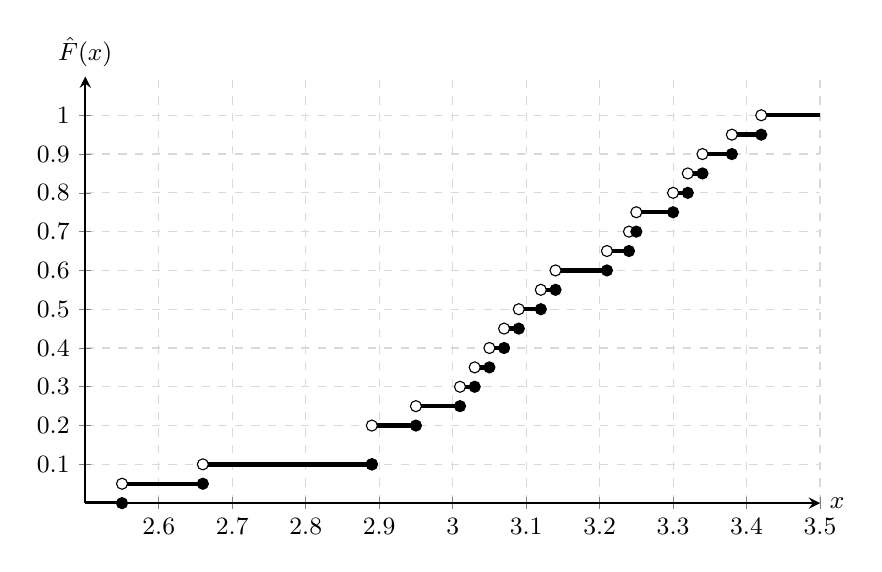
\begin{tikzpicture}
\begin{axis}[
    width=0.9\textwidth, height=7cm,
    axis lines=middle,
    axis line style={thick, black},
    xlabel={$x$},
    ylabel={$\hat{F}(x)$},
    xlabel style={right},
    ylabel style={above},
    ymin=0, ymax=1.1,
    xmin=2.5, xmax=3.5,
    ytick={0, 0.1, ..., 1.1},
    grid=major,
    grid style={dashed, gray!30},
    axis background/.style={fill=white},
    tick label style={font=\small},
    label style={font=\small}
]
\addplot[ultra thick, black, no marks, const plot] coordinates {(2.5, 0) (2.55, 0)};
\addplot[only marks, mark=*, mark options={fill=black}, mark size=2pt] coordinates {(2.55, 0)};
\addplot[ultra thick, black, no marks, const plot] coordinates {(3.42, 1) (3.5, 1)};
\addplot[only marks, mark=*, mark options={fill=white, draw=black}, mark size=2pt] coordinates {(3.42, 1)};
\addplot[ultra thick, black, no marks, const plot] coordinates {(2.55, 0.05) (2.66, 0.05)};
\addplot[only marks, mark=*, mark options={fill=white, draw=black}, mark size=2pt] coordinates {(2.55, 0.05)};
\addplot[only marks, mark=*, mark options={fill=black}, mark size=2pt] coordinates {(2.66, 0.05)};
\addplot[ultra thick, black, no marks, const plot] coordinates {(2.66, 0.1) (2.89, 0.1)};
\addplot[only marks, mark=*, mark options={fill=white, draw=black}, mark size=2pt] coordinates {(2.66, 0.1)};
\addplot[only marks, mark=*, mark options={fill=black}, mark size=2pt] coordinates {(2.89, 0.1)};
\addplot[ultra thick, black, no marks, const plot] coordinates {(2.89, 0.1) (2.89, 0.1)};
\addplot[only marks, mark=*, mark options={fill=white, draw=black}, mark size=2pt] coordinates {(2.89, 0.1)};
\addplot[only marks, mark=*, mark options={fill=black}, mark size=2pt] coordinates {(2.89, 0.1)};
\addplot[ultra thick, black, no marks, const plot] coordinates {(2.89, 0.2) (2.95, 0.2)};
\addplot[only marks, mark=*, mark options={fill=white, draw=black}, mark size=2pt] coordinates {(2.89, 0.2)};
\addplot[only marks, mark=*, mark options={fill=black}, mark size=2pt] coordinates {(2.95, 0.2)};
\addplot[ultra thick, black, no marks, const plot] coordinates {(2.95, 0.25) (3.01, 0.25)};
\addplot[only marks, mark=*, mark options={fill=white, draw=black}, mark size=2pt] coordinates {(2.95, 0.25)};
\addplot[only marks, mark=*, mark options={fill=black}, mark size=2pt] coordinates {(3.01, 0.25)};
\addplot[ultra thick, black, no marks, const plot] coordinates {(3.01, 0.3) (3.03, 0.3)};
\addplot[only marks, mark=*, mark options={fill=white, draw=black}, mark size=2pt] coordinates {(3.01, 0.3)};
\addplot[only marks, mark=*, mark options={fill=black}, mark size=2pt] coordinates {(3.03, 0.3)};
\addplot[ultra thick, black, no marks, const plot] coordinates {(3.03, 0.35) (3.05, 0.35)};
\addplot[only marks, mark=*, mark options={fill=white, draw=black}, mark size=2pt] coordinates {(3.03, 0.35)};
\addplot[only marks, mark=*, mark options={fill=black}, mark size=2pt] coordinates {(3.05, 0.35)};
\addplot[ultra thick, black, no marks, const plot] coordinates {(3.05, 0.4) (3.07, 0.4)};
\addplot[only marks, mark=*, mark options={fill=white, draw=black}, mark size=2pt] coordinates {(3.05, 0.4)};
\addplot[only marks, mark=*, mark options={fill=black}, mark size=2pt] coordinates {(3.07, 0.4)};
\addplot[ultra thick, black, no marks, const plot] coordinates {(3.07, 0.45) (3.09, 0.45)};
\addplot[only marks, mark=*, mark options={fill=white, draw=black}, mark size=2pt] coordinates {(3.07, 0.45)};
\addplot[only marks, mark=*, mark options={fill=black}, mark size=2pt] coordinates {(3.09, 0.45)};
\addplot[ultra thick, black, no marks, const plot] coordinates {(3.09, 0.5) (3.12, 0.5)};
\addplot[only marks, mark=*, mark options={fill=white, draw=black}, mark size=2pt] coordinates {(3.09, 0.5)};
\addplot[only marks, mark=*, mark options={fill=black}, mark size=2pt] coordinates {(3.12, 0.5)};
\addplot[ultra thick, black, no marks, const plot] coordinates {(3.12, 0.55) (3.14, 0.55)};
\addplot[only marks, mark=*, mark options={fill=white, draw=black}, mark size=2pt] coordinates {(3.12, 0.55)};
\addplot[only marks, mark=*, mark options={fill=black}, mark size=2pt] coordinates {(3.14, 0.55)};
\addplot[ultra thick, black, no marks, const plot] coordinates {(3.14, 0.6) (3.21, 0.6)};
\addplot[only marks, mark=*, mark options={fill=white, draw=black}, mark size=2pt] coordinates {(3.14, 0.6)};
\addplot[only marks, mark=*, mark options={fill=black}, mark size=2pt] coordinates {(3.21, 0.6)};
\addplot[ultra thick, black, no marks, const plot] coordinates {(3.21, 0.65) (3.24, 0.65)};
\addplot[only marks, mark=*, mark options={fill=white, draw=black}, mark size=2pt] coordinates {(3.21, 0.65)};
\addplot[only marks, mark=*, mark options={fill=black}, mark size=2pt] coordinates {(3.24, 0.65)};
\addplot[ultra thick, black, no marks, const plot] coordinates {(3.24, 0.7) (3.25, 0.7)};
\addplot[only marks, mark=*, mark options={fill=white, draw=black}, mark size=2pt] coordinates {(3.24, 0.7)};
\addplot[only marks, mark=*, mark options={fill=black}, mark size=2pt] coordinates {(3.25, 0.7)};
\addplot[ultra thick, black, no marks, const plot] coordinates {(3.25, 0.75) (3.3, 0.75)};
\addplot[only marks, mark=*, mark options={fill=white, draw=black}, mark size=2pt] coordinates {(3.25, 0.75)};
\addplot[only marks, mark=*, mark options={fill=black}, mark size=2pt] coordinates {(3.3, 0.75)};
\addplot[ultra thick, black, no marks, const plot] coordinates {(3.3, 0.8) (3.32, 0.8)};
\addplot[only marks, mark=*, mark options={fill=white, draw=black}, mark size=2pt] coordinates {(3.3, 0.8)};
\addplot[only marks, mark=*, mark options={fill=black}, mark size=2pt] coordinates {(3.32, 0.8)};
\addplot[ultra thick, black, no marks, const plot] coordinates {(3.32, 0.85) (3.34, 0.85)};
\addplot[only marks, mark=*, mark options={fill=white, draw=black}, mark size=2pt] coordinates {(3.32, 0.85)};
\addplot[only marks, mark=*, mark options={fill=black}, mark size=2pt] coordinates {(3.34, 0.85)};
\addplot[ultra thick, black, no marks, const plot] coordinates {(3.34, 0.9) (3.38, 0.9)};
\addplot[only marks, mark=*, mark options={fill=white, draw=black}, mark size=2pt] coordinates {(3.34, 0.9)};
\addplot[only marks, mark=*, mark options={fill=black}, mark size=2pt] coordinates {(3.38, 0.9)};
\addplot[ultra thick, black, no marks, const plot] coordinates {(3.38, 0.95) (3.42, 0.95)};
\addplot[only marks, mark=*, mark options={fill=white, draw=black}, mark size=2pt] coordinates {(3.38, 0.95)};
\addplot[only marks, mark=*, mark options={fill=black}, mark size=2pt] coordinates {(3.42, 0.95)};
\end{axis}
\end{tikzpicture}

\caption{Эмпирическая функция распределения $\hat{F}(x)$}
\end{figure}